\section{The Standard Model of Particle Physics}\label{sec:sm}

The SM is formulated as a relativistic quantum field theory (QFT) where each particle in the theory is represented by its own field and excitations of those fields are then the physical particles that we observe in nature. Particles can interact with each other via the exchange of a subset of SM particles called \textit{force carriers}. The types of allowed interactions and their corresponding strengths are encoded in a Lagrangian density, \LSM, together with the particle properties (mass and spin). 

\subsection{Particle Content}
A schematic of the SM particle content, including every SM particle with its properties and categorizations is provided in \cref{fig:sm_particle_content}. The particle content can be initially categorized into two groups: spin-$\frac{1}{2}$ fermions which are matter constituents, and spin-integer bosons which are force carriers and are spin-1 except for the Higgs boson which is spin-0. 

There are four spin-1 bosons in the SM: the photon ($\gamma$) which mediates the electromagnetic force, the \PWpm and \PZ bosons which mediate the weak force, and the gluon (\Pg) which mediates the strong force. Particles that interact with photons carry \textit{electric charge}; particles that interact with gluons carry a \textit{colour charge}, which comes in three possible states: $r$, $g$ and $b$, and particles that interact with \PWpm and \PZ bosons carry charges called \textit{weak isospin} and/or \textit{weak hypercharge}. More details on these charges are given in \cref{sec:sm_lagrangian}.

The fermions are split by those that interact with the strong force, called \textit{quarks}, and those that do not, called \textit{leptons}. Leptons are further split into those which are electrically charged ($l$), and those which are not, called \textit{neutrinos} ($\nu$).  Quarks are similarly split by electric charge into up-type quarks and down-type quarks, with charge $\frac{2}{3}$ and $-\frac{1}{3}$ respectively (in units of elementary charge, $e$). 

The fermions can be also categorized into three generations based on a mass hierarchy, where the first generation is the least massive. Each generation contains an up-type quark, a down-type quark, a charged lepton, and a neutrino. The first generation contains the main constituents of the visible matter in the universe, those being the up and down quarks, and the electron. Additionally, all charged fermions have a corresponding antiparticle which has the same mass but opposite charge and parity.

The remaining particle is the Higgs boson which plays a special role in the SM. We will see later on that its introduction to the model is necessary to correctly describe the distribution of masses for particles in the theory. 

\begin{figure}
  \centering
  \hbox{\hspace{-2.5cm}\resizebox{1.2\textwidth}{!}{\inputtikz{Figures/Theory/SM/particle_content.tex}}}
  \caption[SM Particle Content]{Particle content of the SM. The mass, electric charge, colour and spin are given for each particle. All masses are taken from Ref.~\cite{ParticleDataGroup:2020ssz} except the Higgs boson mass which is taken from Ref.~\cite{CMS:2020xrn}.}\label{fig:sm_particle_content}
\end{figure}
\subsection{Interactions}
The electromagnetic and weak forces are described together by a single force: the \textit{electroweak} force. Particles that interact via the electroweak force include all fermions and the electroweak bosons: \PZ, \PW, $\gamma$ and \PH (all bosons except the gluon). Feynman diagram vertices for these interactions are given in \cref{fig:electroweak_fermion_vertices}. All fermions can interact via the exchange of \PZ boson and all left-handed particles/right-handed anti-particles can interact via the exchange of a \PW boson. All electrically charged fermions can interact via the exchange of a photon and all massive fermions can interact with the Higgs boson. The three and four-point interactions involving only electroweak bosons, shown in \cref{fig:electroweak_3_point_boson_vertices,fig:electroweak_4_point_boson_vertices}, are also allowed. In the strong force, quarks and gluons interact with each other according to the Feynman diagram vertices shown in \cref{fig:strong_vertices}.

\begin{figure}[b!]
  \centering
  \inputtikz{Figures/Theory/SM/ffz.tex}
  \inputtikz{Figures/Theory/SM/ffa.tex}
  \inputtikz{Figures/Theory/SM/ffh.tex} \\
  \inputtikz{Figures/Theory/SM/fnuw.tex}
  \inputtikz{Figures/Theory/SM/udw.tex}
  \caption[Electroweak Feynman Diagram Vertices]{Feynman diagram vertices allowed in the SM involving electroweak interactions with fermions. Interactions with a photon, \PZ boson, or a Higgs boson, require the fermion ($f$) flavour to be the same. Massive fermions are denoted by $f_m$ and exclude neutrinos. Interactions with \PW bosons can involve fermions from different generations and must involve either a lepton ($l$) and a neutrino ($\nu$) or an up-type quark ($u$) and a down-type quark ($d$). The $L$ and $R$ subscripts denote left-handed and right-handed fermions respectively. Charged-conjugated versions of the \PW-interaction diagrams are also possible if the handedness is reversed.}\label{fig:electroweak_fermion_vertices}
\end{figure} 


\begin{figure}
  \centering
  \inputtikz{Figures/Theory/SM/wwz.tex}
  \inputtikz{Figures/Theory/SM/wwh.tex}
  \inputtikz{Figures/Theory/SM/zzh.tex}
  \inputtikz{Figures/Theory/SM/hhh.tex}
  \caption[Three-Point Electroweak Boson Feynman Diagram Vertices]{Feynman diagram vertices allowed in the SM involving three electroweak bosons.}\label{fig:electroweak_3_point_boson_vertices}
\end{figure}

\begin{figure}
  \centering
  \inputtikz{Figures/Theory/SM/wwzz.tex}
  \inputtikz{Figures/Theory/SM/wwww.tex} \\
  \inputtikz{Figures/Theory/SM/wwhh.tex}
  \inputtikz{Figures/Theory/SM/hhhh.tex}
  \caption[Four-Point Electroweak Boson Feynman Diagram Vertices]{Feynman diagram vertices allowed in the SM involving four electroweak bosons.}\label{fig:electroweak_4_point_boson_vertices}
\end{figure}

\begin{figure}
  \centering
  \inputtikz{Figures/Theory/SM/qqg.tex}
  \inputtikz{Figures/Theory/SM/ggg.tex}
  \inputtikz{Figures/Theory/SM/gggg.tex}
  \caption[Strong Feynman Diagram Vertices]{Feynman diagram vertices allowed in the SM that involve a strong interaction. On the left, $q$ refers to a quark (or antiquark) of the same flavour.}\label{fig:strong_vertices}
\end{figure}
\subsection{Quantum Field Theory}\label{sec:electroweak}
The SM can be described by a Lagrangian density, \LSM, which is a function of the particle fields and their derivatives. By applying the Euler-Lagrange equations to \LSM, we can then derive equations of motion that describe the dynamics and interactions of these fields. In this section, concepts related to QFT that will help to understand the construction of \LSM will be described. In the rest of this section, Lagrangian densities will be represented by $\mathcal{L}$ and referred to as ``Lagrangians'' (omitting ``density'').

\subsubsection{Real Scalar Fields}
One of the simplest particle theories one could write down consists of a single Lorentz real scalar field, $\phi(x,y,z,t)$, with a Lagrangian:
\begin{equation}
  \mathcal{L} = \frac{1}{2}\partial_\mu \phi \partial^\mu \phi - \frac{1}{2}m^2\phi^2
\end{equation}
and after applying the Euler-Lagrange equations:
\begin{equation}
  0 = \frac{\partial \mathcal{L}}{\partial \phi} - \partial_\mu \frac{\partial \mathcal{L}}{\partial(\partial_\mu \phi)}
\end{equation}
this becomes:
\begin{equation}
  0 = \partial_\mu \partial^\mu \phi + m^2 \phi \label{eq:klein_gordon}
\end{equation}
which can be identified as a relativistic wave equation, namely the Klein-Gordon equation, which describes a particle with mass $m$. In this theory, the particles are non-interacting. To introduce interactions, we need to add terms that are higher orders of \phi, for example:
\begin{equation}
  \mathcal{L} = \frac{1}{2}\partial_\mu \phi \partial^\mu \phi - \frac{1}{2}m^2\phi^2 + \lambda_3 \phi^3 + \lambda_4 \phi^4
  \label{eq:scalar4}
\end{equation}
where $\lambda_3 \phi^3$ and $\lambda_4 \phi^4$ correspond to three-point and four-point interactions respectively. Generally, a term containing greater than two fields, including powers of the same field, corresponds to an interaction involving that combination of fields. Adding terms that have powers of $\phi$ greater than four are not allowed if one wants a renormalizable theory, i.e.\ a theory that has finite predictions at arbitrarily high energy scales~\cite{Peskin:1995ev}. Strictly speaking, a renormalizable Lagrangian must have dimensions $[\mathcal{L}] = \mathrm{GeV}^4$. Given that $[\partial_\mu \phi] = \mathrm{GeV}^2$, $[\phi] = \mathrm{GeV}$ and $[m] = \mathrm{GeV}$, this is satisfied in \cref{eq:scalar4}. 

\newpage

\noindent
Regardless of renormalizability, a Lagrangian must additionally:
\begin{enumerate}
  \item be real since the action, $S$, which is an integral over the Lagrangian, must be real;
  \item be a local function of the fields and their derivatives calculated at the same spacetime point;
  \item be invariant under any symmetries of the theory.
\end{enumerate}
\Cref{eq:scalar4} is invariant under Poincar\'e transformations, which include translations and rotations in space, as well as Lorentz boosts. According to Noether's theorem, a continuous symmetry has a corresponding conservation law and in the case of Poincar\'e transformations, the conserved quantities are energy, momentum, and angular momentum. The full SM Lagrangian has additional symmetries which will be highlighted throughout the rest of this section.

Lorentz invariance is an assumed requirement for all Lagrangians in this chapter. The condition on renormalization is also required except for effective field theories which will be discussed in \cref{sec:EFT}. 

\subsubsection{Vector Fields}
In the SM, the spin-1 force carriers are represented by vector fields. The most general Lagrangian that is Lorentz invariant and contains a real vector field is:
\begin{equation}
  \mathcal{L} = aS^2 + b F_\mn F^\mn + c G_\mn G^\mn + d A_\mu A^\mu
\end{equation}
where:
\begin{align}
  S &= \partial_\mu A^\mu,\quad &&\text{is a Lorentz scalar}; \\
  F_\mn &= \partial_\mu A_\nu - \partial_\nu A_\mu,\quad &&\text{is an antisymmetric rank 2 tensor}; \label{eq:fmn} \\
  G_\mn &= \partial_\mu A_\nu + \partial_\nu A_\mu - \frac{1}{2} \eta_\mn S,\quad &&\text{is a symmetric and traceless rank 2 tensor};
\end{align}
and $a, b, c$ and $d$ are arbitrary constants. If we want the Lagrangian to also be gauge invariant, meaning that it is invariant under transformations of the form:
\begin{equation}
  A_\mu \to A_\mu - \partial_\mu \lambda
  \label{eq:gauge_transformation}
\end{equation}
where $\lambda$ is an arbitrary scalar function of spacetime, only one of the terms is viable and the most general Lagrangian is:
\begin{equation}
  \mathcal{L} = F_\mn F^\mn .
\end{equation}
This is the Maxwell Lagrangian for the free electromagnetic field.

\subsubsection{Complex Scalar Fields}
Returning to scalar fields but now considering the field to be complex, the most general Lagrangian becomes:
\begin{equation}
  \mathcal{L} = \partial_\mu \phi^* \partial^\mu \phi - V(\phi^*\phi)
  \label{eq:scalar_complex}
\end{equation}
where the potential, $V(\phi^*\phi)$, is a polynomial of order two or less. The three-point interaction term is now missing due to the requirement that $\mathcal{L}$ be real, and the Lagrangian has a new symmetry compared to the real scalar field Lagrangian. The Lagrangian is now invariant under the rotation of a complex phase:
\begin{equation}
  \phi(x) \to e^{i\theta}\phi(x)
\end{equation}
where $\theta$ is a real number. The symmetry is called \textit{Abelian} because the transformations commute:
\begin{equation}
  e^{-i\theta_1}e^{-i\theta_2} = e^{-i\theta_2}e^{-i\theta_1},
\end{equation}
and is called a \textit{global symmetry} because the same transformation is applied at all points in spacetime, i.e.\ $\theta$ is a constant. 

The Lagrangian of \Cref{eq:scalar_complex} is not invariant under a local transformation of the type:
\begin{equation}
  \phi(x) \to e^{i\theta(x)} \phi(x)
  \label{eq:local_transformation}
\end{equation}
but an invariant Lagrangian can be created if a new vector field, $A_\mu$, is introduced which simultaneously transforms as 
\begin{equation}
  A_\mu(x) \to A_\mu(x) - \frac{1}{e}\partial_\mu \theta(x)
  \label{eq:gauge_transformation_2}
\end{equation}
which is the same as the gauge transformation in \cref{eq:gauge_transformation} where $\lambda = \theta(x)/e$. The simultaneous transformation of $\phi$ and $A_\mu$ is referred to as a \textit{local gauge} transformation and the new vector field is known as a \textit{gauge field}. The Lagrangian is given by:
\begin{equation}
  \mathcal{L} = (D_\mu\phi)^* D^\mu \phi - V(\phi^*\phi)
  \label{eq:scalar_complex_gauge}
\end{equation}
where the covariant derivative, $D_\mu$, is defined as:
\begin{equation}
  D_\mu \phi \equiv \partial_\mu \phi + ieA_\mu \phi.
\end{equation}
Now adding the $F_\mn F^\mn$ term (\cref{eq:fmn}), we arrive at the most general gauge invariant Lagrangian for a complex scalar field:
\begin{equation}
  \mathcal{L} = F_\mn F^\mn + (D_\mu\phi)^* D^\mu \phi - V(\phi^*\phi) .
\end{equation}

In the SM, local gauge symmetries are imposed on the Lagrangian which give rise to the existence of vector bosons, which are the force carriers: the gluons, photon, and the \PWpm and \PZ bosons. Given that they are related to gauge transformations, the force carriers are also referred to as \textit{gauge bosons}.

\subsubsection{Non-Abelian Gauge Fields}
The simultaneous transformation of $\phi$ and $A_\mu$ in \cref{eq:local_transformation,eq:gauge_transformation_2} is a \U{1} transformation. When generalizing to \U{N}, the Lagrangian in \cref{eq:scalar_complex_gauge} becomes:
\begin{equation}
  \mathcal{L} = (D_\mu\phi)^\dag D^\mu \phi - V(\phi^\dag\phi)
\end{equation}
where $\phi$ and $A_\mu$ transform as
\begin{align}
  \phi &\to M \phi \\
  A_\mu &\to M A_\mu M^\dag + \frac{i}{g}(\partial_\mu M)M^\dag \label{eq:non_abelian_vector_transformation}
\end{align}
where $M(x)$ is an element of the \U{N} group. \Cref{eq:non_abelian_vector_transformation} holds if $A_\mu$ is an element of the Lie algebra, meaning that it can be written as $A_\mu = A_\mu^a T^a$ where $A_\mu^a$ are real constants, $T^a$ are the generators of some representation of the Lie algebra, and $a \in \{1,\ldots,D\}$ where $D=N^2$ is the dimensionality of \U{N}. Therefore, imposing a local \U{N} symmetry has lead to the introduction of $D$ gauge bosons, where each gauge boson is represented by a component, $A_\mu^a$. 

In the non-Abelian case, the $F_\mn F^\mn$ term is no longer gauge invariant. In an attempt to find a similar term that \textit{is} gauge invariant, we redefine $F_\mn$ as:
\begin{align}
  F_\mn &= -\frac{i}{g} [D_\mu, D_\nu] \\
  &= \partial_\mu A_\nu - \partial_\nu A_\mu + ig[A_\mu, A_\nu]
\end{align}
which is still consistent with the Abelian case since $[A_\nu, A_\nu]$ would be zero. With this definition, $F_\mn F^\mn$ is still not invariant, but its trace is. Therefore, the most general scalar field Lagrangian with a \U{N} gauge symmetry is:
\begin{equation}
  \mathcal{L} = -\frac{1}{2} \Tr F_\mn F^\mn + (D_\mu\phi)^\dag D^\mu \phi - V(\phi^\dag\phi).
\end{equation}

Writing the first term alone and in terms of the gauge field components, $A_\mu^a$, we find:
\begin{align}
  \mathcal{L} = &-\frac{1}{2} \Tr F_\mn F^\mn = - \frac{1}{4} F_\mn^a F^{\mn a} \\
  &= -\frac{1}{4} (\partial_\mu A_\nu^a - \partial_\nu A_\mu^a) (\partial_\nu A^a_\mu) (\partial^\mu A^{\nu a} - \partial^\nu A_{\mu a}) (\partial_\nu A^a_\mu) \\
  &+ \frac{g}{2} f^{abc} (\partial_\mu A^a_\nu - \partial_\nu A^a_\mu) A^{\mu b}A^{\nu c} - \frac{g^2}{4} f^{abc} f^{ade} A_\mu^b A_\nu^c A^{\mu d} A^{\nu e}
\end{align}
where the last two terms represent three-point and four-point interactions of the gauge bosons, in an analogous way to \cref{eq:scalar4}. 

The conclusions reached here about non-abelian gauge fields apply to any subset of \U{N}, including \SU{N} groups which are seen in the SM.

\subsubsection{Spinors}
In addition to the Klein-Gordon equation (\cref{eq:klein_gordon}), particles that have spin $\frac{1}{2}$ must also satisfy the Dirac equation:
\begin{equation}
  i \gamma^\mu \partial_\mu \psi - m \psi = 0
\end{equation}
where $m$ is the mass of the particle, $\psi$ is the particle field, and $\gamma^\mu$ are the $4\times4$ gamma matrices~\cite{Thomson:2013zua}. 

A Lorentz scalar that can be constructed out of spinor fields is $\bar{\psi} \psi$ where we have introduced the Dirac adjoint, $\bar{\psi}$, as: 
\begin{equation}
  \bar{\psi} \equiv \psi^\dag \gamma^0 .
\end{equation}
For any pair of spinors, $\psi$ and $\chi$, $\bar{\psi} \gamma^\mu \chi$ is a Lorentz vector, and for any Lorentz vector, $a_\mu$, $\bar{\psi} \slashed{a} \chi$ is a Lorentz scalar where we have introduced the Dirac slash notation:
\begin{equation}
  \slashed{a} \equiv \gamma^\mu a_\mu .
\end{equation}
This also applies when the vector is a derivative so $\bar{\psi}\slashed{\partial}\psi$ is also a Lorentz scalar.

In the SM, spinors are decomposed into their left and right-handed components. To define these components, we first introduce a fifth gamma matrix:
\begin{equation}
  \gamma^5 = i\gamma^0 \gamma^1 \gamma^2 \gamma^3 .
\end{equation}
The left/right-handed component of a spinor, $\psi_{L/R}$, is given by $P_{L/R} \psi$ where:
\begin{equation}
  P_L = \frac{1}{2} (\iden - \gamma^5) \text{ and } P_R = \frac{1}{2}(\iden + \gamma^5) .
\end{equation}
Under a parity transformation, a left/right-handed spinor transforms as:
\begin{equation}
  \psi_{L/R} \to \gamma^0 \psi_{L/R}
\end{equation}
and it can be shown that $P_{L/R} (\gamma^0 \psi_{L/R}) = 0$, i.e.\ a parity transformation changes a left-handed spinor into a right-handed spinor and a right-handed spinor into a left-handed spinor. Given this transformation property, we can create a parity-violating theory by writing a Lagrangian that has different terms for $\psi_L$ than for $\psi_R$. This will be essential in describing the weak interaction that behaves differently with left and right-handed fermions.

\subsubsection{Spontaneous Symmetry Breaking}
So far, we have interpreted a field, $\phi$, in a Lagrangian as the field of a physical particle. This has the implicit assumption that a field value of zero corresponds to the vacuum state of the Lagrangian, i.e.\ the state with the lowest energy. However, this need not be the case. Consider the complex scalar Lagrangian of \cref{eq:scalar_complex}, which has a global \U{1} symmetry, with the potential:
\begin{equation}
  V(\phi^*, \phi) = m^2 \phi^*\phi + \frac{1}{2}\lambda (\phi^*\phi)^2 .
  \label{eq:scalar_complex_potential}
\end{equation}
\begin{figure}
  \centering
  \scalebox{1.5}{
   \inputtikz{Figures/Theory/SM/sombrero.tex}
  }
  \caption[Higgs Field Potential]{The potential of a complex scalar field, $V(\phi) = m^2 \phi^*\phi + \frac{1}{2}\lambda (\phi^*\phi)^2$, where $m^2 < 0$ and $\lambda > 0$.}\label{fig:sombrero}
\end{figure}
If $m^2 < 0$ and $\lambda > 0$, then the potential will look like that shown in \cref{fig:sombrero} and have a circle of minima in the complex plane at:
\begin{equation}
  \phi = \frac{v}{\sqrt{2}}e^{i\theta},\quad \theta \in [0, 2\pi]
  \label{eq:phi_vacuum_state}
\end{equation}
where we have used the conventions, $\mu^2 = -m^2$ and $v = \mu / \sqrt{\lambda}$, where $v$ is real and referred to as the \textit{vacuum expectation value} (vev). We can choose a particular minimum, $\phi = \phi_0 = v / \sqrt{2}$, and expanding around this vacuum state we get:
\begin{alignat}{2}
  \phi (x) &= \frac{1}{\sqrt{2}} (v + \rho(x) ), \quad &&\rho \in \mathbb{C} \\
  &= \frac{1}{\sqrt{2}} (v + \varphi (x) + i \chi (x) ), \quad &&\varphi,\chi \in \mathbb{R}
\end{alignat}
and the potential becomes:
\begin{equation}
  V(\phi^*, \phi) = -\frac{\mu^4}{2\lambda} + \mu^2 \varphi^2 + \frac{1}{2} \lambda v \varphi (\varphi^2 + \chi^2) + \frac{1}{8} \lambda (\varphi^2 + \chi^2)^2
  \label{eq:scalar_complex_potential_expanded}
\end{equation}
where the second term is a mass term for $\varphi$ and there are no mass terms for $\chi$. By expanding around the vacuum state, we have revealed the physical particle spectrum for this Lagrangian, which is two scalar particles, $\varphi$ and $\chi$, where $m_\varphi = \sqrt{2}\mu$ and $\chi$ is massless. The massless scalar particle is known as a Goldstone boson.



This Lagrangian is invariant under a global \U{1} transformation: $\phi \to e^{i\theta} \phi$, but since $e^{i\theta}\phi_0 \neq \phi_0$, this does not correspond to the analogous transformation: $\rho \to e^{i\theta} \rho$. We therefore say that the global \U{1} symmetry is \textit{spontaneously broken}. The original symmetry is still present, but not apparent now that the Lagrangian is written in terms of the physical particle fields. 

We can now generalize to theories that are invariant under any symmetry group, $G$, whereby the field transforms as $\phi \to M \phi$, where $M$ is an element of the group. The symmetry is spontaneously broken if $M \phi_0 \neq \phi_0$ for any $M$, or unbroken if $M \phi_0 = \phi_0$ for all $M$. Considering an infinitesimal transformation of $\phi_0$:
\begin{equation}
  \phi_0 \to \phi_0 + i \theta^a T^a \phi_0
\end{equation}
where $T^a$ are the generators of the group, and $\theta^a$ are infinitesimally-small real constants, we identify broken generators as ones where $T \phi_0 \neq \phi_0$ and unbroken generators as ones where $T \phi_0 = \phi_0$. The set of unbroken generators corresponds to a \textit{residual symmetry group}, $H$, which is a subgroup of the original group. 

When $T \phi \neq 0$ for all $T$, there may still exist linear combinations of the generators, $\hat{T}=c^a T^a$ where $\hat{T} \phi_0 = 0$. To determine these linear combinations, we first define the symmetry breaking matrix:
\begin{equation}
  S^{ab} = \phi_0^\dag \{T^a, T^b\} \phi_0 .
  \label{eq:symmetry_breaking_matrix}
\end{equation}
For \U{N} and \SU{N} symmetry groups where $T^a$ are Hermitian, $S^{ab}$ is real and symmetric and therefore has $D$ real eigenvectors, $c_i$, with eigenvalues $\lambda_i$. It can be shown that a new generator defined as $\hat{T}^i = c_i^a T^a$, is an unbroken generator when $\lambda_i = 0$, and a broken generator when $\lambda_i \neq 0$. It can be further shown that every broken generator gives rise to a massless Goldstone particle. This is known as Goldstone's theorem~\cite{Goldstone:1962es} and holds for theories with global symmetries. To determine the particle spectra of a gauge theory, we turn to the Higgs mechanism.

\subsubsection{The Higgs Mechanism}
Consider the Lagrangian of \cref{eq:scalar_complex_gauge}, which has a local \U{1} symmetry, with the same potential as \cref{eq:scalar_complex_potential}. Now that the vector field, $A^\mu$, is introduced, the vacuum state is specified by values of $A^\mu$ and $\phi$ simultaneously. In the temporal gauge ($A^0 = 0$), this is given by \cref{eq:phi_vacuum_state} and $A_\mu = 0$.
  
Once again expanding the scalar field as $\phi = (v + \varphi + i \chi) / \sqrt{2}$, we regain the same potential as \cref{eq:scalar_complex_potential_expanded} and new terms from the expansion of $F_\mn F^\mn$ and $(D_\mu \phi)^* D^\mu \phi$. Writing only the quadratic terms and transforming to the unitary gauge ($\theta(x) = -\chi / v$) we find:
\begin{equation}
  \mathcal{L} = F_\mn F^\mn + \frac{1}{2} e^2 v^2 A_\mu A^\mu + \frac{1}{2} \partial_\mu \varphi \partial^\mu \varphi - \mu^2 \varphi^2 + \cdots
\end{equation}
where we can identify two distinct fields, $A_\mu$ and $\phi$, which have masses $\sqrt{2}\mu$ and $ev$ respectively. As in the global case, the \U{1} symmetry is broken, but unlike the global case, the symmetry breaking has not led to any massless particles. Instead, the originally-massless vector boson has been given a mass.

When generalizing to theories that are invariant under any symmetry group, a similar conclusion is found. If there are $D$ generators of the group, where $D^'$ are broken, then there are $D^'$ massive vector particles and $D-D^'$ massless vector bosons. In the SM, this is the mechanism by which the gauge bosons of the weak force, \PWpm and \PZ, acquire mass. 
\subsection{The Standard Model Lagrangian}\label{sec:sm_lagrangian}
\subsubsection{Quantum Electrodynamics}
The QFT of electromagnetism is known as quantum electrodynamics (QED). It describes the interaction between charged fermions and photons which are represented by a spinor, $\psi$, and a vector field, $A^\mu$, respectively. The QED Lagrangian is:
\begin{equation}
  \LQED = -\frac{1}{4} F_\mn F^\mn +  \bar{\psi} (i \slashed{D} - m)\psi,
\end{equation}
and is invariant under global and local \U{1} transformations which lead to the conservation of particle number and electric charge respectively. It also is symmetrical under parity, charge conjugation, and time reversal transformations. However, experiments have shown that parity symmetry is only approximate, and can be violated~\cite{Wu:1957my}. Therefore, the QED Lagrangian does not sufficiently describe the behaviour of charged fermions in nature. In the SM, parity violation is introduced via the weak force which couples only to left-handed fermions.

We can start to consider how we can introduce parity violation by writing the fermionic components of the QED Lagrangian in terms of the left and right-handed components of the fermion:
\begin{equation}
  \LQED = \bar{\psi}_L i \slashed{\partial} \psi_L + \bar{\psi}_R i \slashed{\partial} \psi_R - m (\bar{\psi}_L \psi_R + \bar{\psi}_R \psi_L) .
\end{equation}
If the fermion is massless, then the left-handed and right-handed components are decoupled from each other and we can write a Lagrangian containing only a left-handed spinor:
\begin{equation}
  \mathcal{L} = \bar{\psi}_L i \slashed{\partial} \psi_L + \cdots
\end{equation}
which would be parity-violating. Therefore, parity violation can be introduced by treating left-handed and right-handed fermions differently in the SM, and this is done in electroweak theory which supersedes QED as a description of electromagnetism and describes the weak interaction at the same time.

\subsubsection{Quantum Chromodynamics}
The QFT of the strong interaction is known as quantum chromodynamics (QCD). The Lagrangian is required to be invariant under local \SU{3} transformations which implies the existence of eight gauge bosons called gluons. The Lagrangian is given by:
\begin{equation}
  \LQCD = \sum_f i \bar{\psi}^f_i (\slashed{D}_{ij} -m^f \delta_{ij})\psi^f_j - \frac{1}{4} G^{c\mn} G^c_\mn
  \label{eq:qcd_lagrangian}
\end{equation}
and the covariant derivative is written as:
\begin{equation}
  (D_\mu)_{ij} = \partial_\mu \delta_{ij} + i g_s G^c_\mu \frac{\lambda^c_{ij}}{2}
\end{equation}
where the strength of the interaction is characterized by $g_s$, the gluons are represented by $G^a_\mu$, and $\lambda^c$ are the Gell-Mann matrices which are a set of $3\times3$ matrices that generate \SU{3}~\cite{Thomson:2013zua}. The quark spinors are given by $\psi^f_i$ where $f \in \{u, d, c, s, t, b\}$ corresponds to a quark \textit{flavour} and $i \in \{r, g, b\}$ corresponds to a quark \textit{colour}. 

Since the \SU{3} symmetry is non-abelian, the gluons are self-interacting and this has profound consequences for the strong interaction. Firstly, $g_s$ increases as the energy scale of an interaction decreases (see \cref{fig:alphas_running}) which is opposite to the behaviour seen in the electromagnetic interaction where there are no self-interactions. This means that at energy scales below $O(1\GeV)$ where $g_s \sim 1$, calculations using perturbation theory are no longer possible, making predictions from QCD more challenging. Fortunately, for energies $O(>100\GeV)$ such as those probed by the LHC, $g_s \sim 0.1$ and perturbation theory is applicable.

A further consequence of gluon self-interactions is the concept of colour confinement which means that quarks and gluons cannot be observed as isolated free particles. Instead, they must exist within colourless bound states called hadrons. States with even and odd numbers of quarks are called mesons and baryons respectively. The two-quark and three-quark variants of these states are commonly produced by QCD interactions at the LHC, and states with higher than three quarks such as tetraquarks and pentaquarks have also been observed~\cite{Liu:2019zoy}.

\begin{figure}
  \centering
  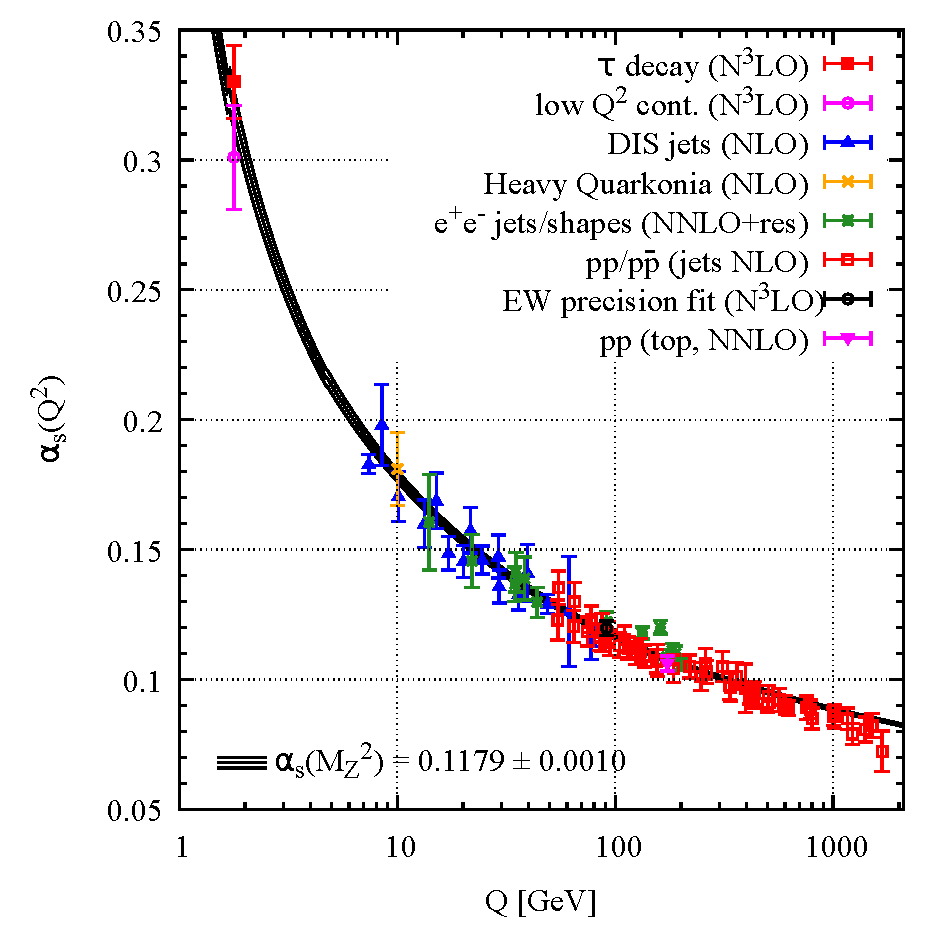
\includegraphics[width=0.7\textwidth]{Figures/Theory/SM/alphas_running.pdf}
  \caption[Measurements of $\alpha_s$ as a Function of Energy Scale]{Summary of measurements of $\alpha_s$ ($\alpha_s = g_s^2 / 4\pi$) as a function of the energy scale, $Q$, taken from Ref.~\cite{ParticleDataGroup:2020ssz}. Each set of coloured points corresponds to a different set of measurements and the degree of QCD perturbation theory used to extract $\alpha_s$ is indicated by the brackets in the legend. Further details about the measurements and $\alpha_s$ calculations can be found in Ref.~\cite{ParticleDataGroup:2020ssz}.}\label{fig:alphas_running}
\end{figure}

\subsubsection{Electroweak Gauge Theory}
In the SM, the electroweak bosons arise from an $\SU{2} \times \U{1}$ gauge symmetry of \LSM. The representation of some field, $\chi$, under \SU{2} is given by generators $\{T^a\}$, $a \in \{1,2,3\}$, and the generator of \U{1} can be any real number, $Y$, such that a gauge transformation is given by:
\begin{equation}
  \chi \to e^{i\theta^a T^a + i\eta Y} \chi
\end{equation}
where $\theta^a$ and $\eta$ are real numbers. The generators $T^a$ and $Y$ are called \textit{weak isospin} and \textit{weak hypercharge} respectively. The covariant derivative is given by:
\begin{equation}
  D_\mu = \partial_\mu + i g_2 A^a_\mu T^a + i g_1 Y B_\mu
  \label{eq:electroweak_covariant}
\end{equation}
where $A^a_\mu$ and $B_\mu$ are the \SU{2} and \U{1} gauge fields respectively. 

Experiments have measured the mass of the \PW and \PZ bosons to be non-zero~\cite{ParticleDataGroup:2020ssz} and in the SM, these masses are introduced via the Higgs mechanism. This necessitates electroweak theory to include a complex scalar field, $\phi$, which is the \textit{Higgs field}, and is in the fundamental representation of \SU{2} and $Y = 1/2$. By defining a fourth generator:
\begin{equation}
  t^4 = \frac{g_1}{2g_2} \iden,
\end{equation}
and $A_\mu^4 = B_\mu$, the gauge fields can be represented by a single vector field in the covariant derivative of the Higgs field:
\begin{equation}
  D_\mu \phi = \partial_\mu \phi + i g_2 A_\mu^{a'} t^{a'} \phi,
\end{equation}
which is useful for applying the ideas of the symmetry breaking matrix introduced in \cref{eq:symmetry_breaking_matrix}. The Lagrangian of the theory is:
\begin{equation}
  \mathcal{L} = -\frac{1}{2} \Tr W_\mn W^\mn - \frac{1}{4} F_\mn F^\mn + (D_\mu \phi)^\dag D^\mu \phi + \mu^2 \phi^\dag \phi - \lambda (\phi^\dag \phi)^2 
  \label{eq:electroweak_gauge_terms}
\end{equation}
where $W_\mn$ and $F_\mn$ are the field strength tensors of the \SU{2} and \U{1} gauge fields respectively. After electroweak symmetry breaking, the residual symmetry group is \U{1} and in terms of the original gauge fields, the physical gauge boson spectrum is:
\begin{align}
  \mathcal{A}_\mu &= \cos{\theta_W} B_\mu + \sin{\theta_W} A^3_\mu, &&\text{ with mass } m_\gamma = 0 \\
  W_\mu^\pm &= \frac{1}{\sqrt{2}} (A^1_\mu \mp i A^2_\mu), &&\text{ with mass } m_\PW = \frac{g_2 v}{2} \\
  Z_\mu &= \cos{\theta_W} A^3_\mu - \sin{\theta_W} B_\mu, &&\text{ with mass } m_\PZ = \frac{v}{2} \sqrt{g_1^2 + g_2^2 } 
\end{align}
which are the photon, \PWpm bosons, and \PZ boson respectively where $\theta_W$ is the Weinberg angle, and is related to $g_1$ and $g_2$ by:
\begin{equation}
  \sin{\theta_W} = \frac{g_1}{\sqrt{g_1^2 + g_2^2 }}\quad \text{and} \quad \cos{\theta_W} = \frac{g_2}{\sqrt{g_1^2 + g_2^2}} .
\end{equation}
In addition, the Higgs field gives rise to a physical scalar boson, the Higgs boson, with mass ${m_H = \sqrt{2} \mu}$. 

In the physical mass basis, the covariant derivative is written as:
\begin{equation}
  D_\mu = \partial_\mu + i \frac{g_1 g_2}{\sqrt{g_1^2 + g_2^2}}(T^3 + Y)\mathcal{A}_\mu + i \frac{g_2^2 T^3 - g_1^2 Y}{\sqrt{g_1^2 + g_2^2}} \PZ_\mu + \frac{ig_2}{\sqrt{2}} (\PW_\mu^+ T^+ + W_\mu^- T^-)
\end{equation}
where $T^\pm = T^1 \pm iT^2$. From the second term, we see that the electric charge, $e$, which characterizes the strength of interactions with photons, is given by:
\begin{equation}
  e = \frac{g_1 g_2}{\sqrt{g_1^2 + g_2^2}} = g_2 \sin{\theta_W} .
\end{equation}
The Weinberg angle can be determined by the ratio of the \PW and \PZ masses:
\begin{equation}
  \cos{\theta_W} = \frac{m_\PW}{m_\PZ} \approx \frac{80.377\GeV}{91.188\GeV} = 0.88145 \pm 0.00013 .
\end{equation}
The parameter, $e$, can be determined from the fine structure constant, $\alpha$:
\begin{equation}
  e = \sqrt{4\pi \alpha} \approx \sqrt{\frac{4\pi}{137}} \approx 0.30
\end{equation}
and the \SU{2} and \U{1} gauge couplings are:
\begin{equation}
  g_2 = \frac{e}{\sin{\theta_W}} \approx 0.64,\quad g_1 = \frac{e}{\cos{\theta_W}} \approx 0.34
\end{equation}
The Higgs vev, $v$, can be determined by the \PW boson mass:
\begin{equation}
  v = \frac{2m_\PW}{g_2} \approx 246\GeV
\end{equation}
and given a measurement of the Higgs boson mass, ${m_\PH = 125.38 \pm 0.14}$~\cite{CMS:2020xrn}, the Higgs self-coupling is determined:
\begin{equation}
  \lambda = \frac{m_H^2}{2v^2} \approx 0.13 .
  \label{eq:higgs_self_coupling}
\end{equation}

\subsubsection{Electroweak Interactions with Fermions}
The interactions of the fermions with the electroweak force are determined by the representation that the fermions take under the \SU{2} and \U{1} gauge transformations. Initially, we will consider only the first generation of fermions: the electron ($e$) and electron neutrino ($\nu$), and the up ($u$) and down ($d$) quarks. Since the weak interaction can change leptons into neutrinos and up into down quarks, left-handed fermions are written in doublets which are in the fundamental representation of \SU{2}:
\begin{equation}
  l_L = \begin{pmatrix}
    \nu_L \\ e_L 
  \end{pmatrix},\quad
  q_L = \begin{pmatrix}
    u_L \\ d_L
  \end{pmatrix}.
\end{equation}
The generators of \U{1}, $Y$, take the value of $-1/2$ and $1/6$ for the left-handed leptons and quarks respectively, where these values are determined by requiring that the fermions have the correct electric charges. Given that the right-handed fermions do not interact with the weak force, they are said be neutral under \SU{2} meaning they do not transform under \SU{2} and the corresponding generator is zero. Additionally, the right-handed neutrino is neutral under \U{1} since it has no electric charge. Therefore, it does not interact with any SM forces, and consequently, it is left out of the theory. The rest of the right-handed fermions are written as singlets, denoted by $e_R$, $u_R$ and $d_R$ and have $Y = -1, 2/3, \text{ and } -1/3$ respectively.

Terms involving fermions and the covariant derivative, referred to as kinetic terms, encode electroweak interactions in the Lagrangian and are:
\begin{equation}
  \LEW = \bar{l}_L i \slashed{D} l_L + \bar{e}_R i \slashed{D} e_R + \bar{q}_L i \slashed{D} q_L + \bar{u}_R i \slashed{D} u_R + \bar{d}_R i \slashed{D} d_R + \cdots
\end{equation}
where $D$ is the covariant derivative defined in \cref{eq:electroweak_covariant}. We must also add terms that encode the mass of the fermions. Since the left-handed and right-handed fermions transform differently under \SU{2} and \U{1}, mass terms like:
\begin{equation}
  -m(\bar{e}_L e_R + \bar{e}_R e_L)
\end{equation} 
are not gauge invariant and cannot be included in \LSM. Instead, the fermion masses are introduced via the Higgs field and spontaneous symmetry breaking similarly to how the gauge bosons acquired their masses. This is achieved with \textit{Yukawa} terms:
\begin{equation}
  \LEW = - y_e (\bar{l}_l \phi l_R + \bar{l}_R \phi^\dag l_L) -  y_u (\bar{q}_L \tilde{\phi} u_R + \bar{u}_R \tilde{\phi}^\dag q_L) - y_d (\bar{q}_l \phi d_R + \bar{q}_R \phi^\dag d_L) + \cdots
\end{equation}
where $y$ are real constants called \textit{Yukawa} couplings and $\tilde{\phi} \equiv i \sigma_2 \phi^*$. After spontaneous symmetry breaking, these terms become:
\begin{equation}
  \LEW = -\frac{y_e v}{\sqrt{2}}  (\bar{e}_L e_R + \bar{e}_R e_L) -\frac{y_u v}{\sqrt{2}}  (\bar{u}_L u_R + \bar{u}_R u_L) -\frac{y_d v}{\sqrt{2}}  (\bar{d}_L d_R + \bar{d}_R d_L) + \cdots
\end{equation}
which corresponds to masses of $y_e v / \sqrt{2}$, $y_u v / \sqrt{2}$ and $y_d v / \sqrt{2}$ for the electron and up and down quarks respectively. No mass term is given to the neutrino and it is therefore massless in the SM. Given the observation of neutrino oscillations~\cite{Super-Kamiokande:1998kpq}, we know that neutrinos are, in fact, not massless in nature, however, for the results discussed in the rest of this thesis, the neutrino masses are small enough that $m_\nu = 0$ is a safe assumption. Therefore, neutrino masses will not be discussed further.

Generalizing to three generations, we define three-component column vectors:
\begin{equation}
  L_L = \begin{pmatrix}
    l_L^1 \\
    l_L^2 \\
    l_L^3 
  \end{pmatrix}, \quad
  L_R = \begin{pmatrix}
    l_R^1 \\
    l_R^2 \\
    l_R^3 
  \end{pmatrix}, \quad
  Q_L = \begin{pmatrix}
    q_L^1 \\
    q_L^2 \\
    q_L^3
  \end{pmatrix}, \quad
  D_R = \begin{pmatrix}
    d_R^1 \\
    d_R^2 \\
    d_R^3 \\
  \end{pmatrix}, \quad
  U_R = \begin{pmatrix}
    u_R^1 \\
    u_R^2 \\
    u_R^3
  \end{pmatrix}
\end{equation}
and then write the kinetic and Yukawa terms as:
\begin{equation}
  \begin{gathered}
    \LEW = \bar{L}_L i \slashed{D} L_L + \bar{L}_R i \slashed{D} L_R + \bar{Q}_L i \slashed{D} Q_L + \bar{D}_R i \slashed{D} D_R + \bar{U}_R i \slashed{D} U_R \\
  - (\bar{L}_L Y_l \phi L_R + \bar{Q}_L Y_d \phi D_R + \bar{Q}_L Y_u \tilde{\phi} U_R + \text{h.c.}) + \cdots
  \end{gathered}
  \label{eq:electoweak_fermion_terms}
\end{equation}
where $Y_{l,d,e}$ are complex $3 \times 3$ Yukawa matrices and $\text{h.c.}$ corresponds to the Hermitian conjugate. By redefining the fermion fields such that the Yukawa matrices are diagonal, we can find the physical mass basis for the fermions. The fields would be redefined according to:
\begin{equation}
  \begin{gathered}
    L_L \to V_{lL} L_L, \quad L_R \to V_{lR} L_R, \quad U_R \to V_{uR}  U_R, \quad  D_R \to V_{dR} D_R, \\
  Q_L = \begin{pmatrix}
    U_L \\
    D_L   
  \end{pmatrix} \to 
  \begin{pmatrix}
    V_{uL} U_L \\
    V_{dL} D_L
  \end{pmatrix}
  \end{gathered}
  \label{eq:fermion_redefinitions}
\end{equation}
where the $V$ matrices are determined by singular value decomposition of the Yukawa matrices. For the leptons, this leaves the kinetic terms:
\begin{equation}
  \LEW =  \sum_f \bar{l}_L^f i \slashed{D} l_L + \bar{l}_R^f i \slashed{D} l_R^f + \cdots
\end{equation}
where $f \in \{e, \mu, \tau\}$, unchanged. Since the terms are the same across flavour, the leptons interact identically in the SM, and this is known as \textit{lepton universality}. Furthermore, the terms are invariant under transformations of the type:
\begin{equation}
  l_L^f \to e^{i\theta^f} l_L^f, \quad l_R^f \to e^{i\theta^f} l_R^f, \quad \theta^f \in \mathbb{R}
\end{equation}
meaning that there is a global $\U{1}_e \times \U{1}_\mu \times \U{1}_\tau$ symmetry. This symmetry corresponds to a conserved lepton number for each generation.

After the field redefinitions of \cref{eq:fermion_redefinitions}, the kinetic terms for the right-handed quarks remain the same in an analogous way to the leptons. However, the kinetic terms for the left-handed quarks do not if $V_{uL} \neq V_{dL}$. When writing the covariant derivative in the physical mass basis, we find that the photon and \PZ boson terms are the same as before. Therefore, interactions with photons and \PZ bosons are identical across quark generation. On the other hand, the \PW boson terms are changed. In terms of the redefined quark fields, the kinetic \PW boson term is:
\begin{equation}
  \LEW = - \frac{g_2}{\sqrt{2}} ( V^{fg}_{\text{CKM}} \bar{u}_L^f \gamma^\mu W_\mu^+ d_L^g + \text{h.c.} ) + \cdots
\end{equation}
where $V_{\text{CKM}} \equiv V_{uL}^\dag V_{dL}$ is the Cabibbo-Kobayashi-Maskawa (CKM) matrix. If $V_{\text{CKM}}$ is not diagonal, it allows the interaction between left-handed quarks and the \PW boson to change quark flavour. There are four free parameters of the CKM matrix which are three mixing angles: $\theta_{12}$, $\theta_{13}$, $\theta_{23}$, and a complex phase: $\delta$. These parameters have been measured and the corresponding CKM matrix is given by:
\begin{equation}
  V_{\text{CKM}} \approx
  \begin{pmatrix}
    0.974 & 0.227 & 0.004 \\
    0.226 & 0.973 & 0.041 \\
    0.009 & 0.040 & 0.999
  \end{pmatrix}
\end{equation}
where the magnitudes of each element, $|V_{\text{CKM}}^{fg}|$, are shown. This indicates that there are small levels of mixing between neighbouring generations, and even smaller mixing between the first and third generations.

The full electroweak Lagrangian is given by the combination of the gauge terms in \cref{eq:electroweak_gauge_terms} with the fermion terms in \cref{eq:electoweak_fermion_terms}:
\begin{align}
  \begin{split}
   \LEW = &-\frac{1}{2} \Tr W_\mn W^\mn - \frac{1}{4} F_\mn F^\mn \\ 
    &+ (D_\mu \phi)^\dag D^\mu \phi + \mu^2 \phi^\dag \phi - \lambda (\phi^\dag \phi)^2 \\
    &+ \bar{L}_L i \slashed{D} L_L + \bar{L}_R i \slashed{D} L_R + \bar{Q}_L i \slashed{D} Q_L + \bar{D}_R i \slashed{D} D_R + \bar{U}_R i \slashed{D} U_R \\
    &- (\bar{L}_L Y_l \phi L_R + \bar{Q}_L Y_d \phi D_R + \bar{Q}_L Y_u \tilde{\phi} U_R + \text{h.c.}) .
  \end{split}
  \label{eq:ew_lagrangian}
\end{align}

\subsubsection{The Standard Model Lagrangian}
To write the full SM Lagrangian, we combine \LEW with \LQCD to get:
\begin{align}
  \begin{split}
    \LSM = &- \frac{1}{4} G^{c\mn} G^c_\mn -\frac{1}{2} \Tr W_\mn W^\mn - \frac{1}{4} F_\mn F^\mn \\ 
    &+ (D_\mu \phi)^\dag D^\mu \phi + \mu^2 \phi^\dag \phi - \lambda (\phi^\dag \phi)^2 \\
    &+ \bar{L}_L i \slashed{D} L_L + \bar{L}_R i \slashed{D} L_R + \bar{Q}_L i \slashed{D} Q_L + \bar{D}_R i \slashed{D} D_R + \bar{U}_R i \slashed{D} U_R \\
    &- (\bar{L}_L Y_l \phi L_R + \bar{Q}_L Y_d \phi D_R + \bar{Q}_L Y_u \tilde{\phi} U_R + \text{h.c.})
  \end{split}
\end{align}
where the covariant derivative is:
\begin{equation}
  D_\mu = \partial_\mu + ig_s G^c_\mu \frac{\lambda^c}{2} + ig_2 A^a_\mu T^a + ig_1 Y B_\mu,
\end{equation}
and where the quark mass terms in \LQCD have been dropped since they are now accounted for with the Yukawa terms. In addition to the 18 free parameters mentioned already, there is also the strong CP phase, $\theta^{\text{CP}}$, that can lead to CP violation in the strong interaction. Experimentally, $\theta^{\text{CP}}$, is known to be very small, $\theta^{\text{CP}} \simeq 0$. More information about this parameter can be found in Ref.~\cite{Wu:1991rw}. All 19 free parameters of the SM are listed in \cref{tab:SM_free_parameters}.

\begin{table}
  \centering
  \begin{tabular}{r|l}
    \toprule
    Fermion masses & $m_u, m_c, m_t, m_d, m_s, m_b, m_e, m_\mu, m_\tau$ \\
    Gauge couplings & $g_s, g_1, g_2$ \\
    Higgs & $\lambda, \mu^2$ \\
    CKM & $\theta_{12}, \theta_{13}, \theta_{23}, \delta$ \\
    Strong CP phase & $\theta^{\text{CP}} (\approx 0)$ \\
    \bottomrule
  \end{tabular}
  \caption[Free Parameters in the SM]{The 19 free parameters of the SM.}\label{tab:SM_free_parameters}
\end{table}
